%!TEX root = main.tex
\section{Policy Gradient}
\subsection{Methodology}
The ultimate goal of policy-based reinforcement learning is to maximize the 
expected cumulative rewards $\textbf{E}_{a \sim Q(a|s)}[R(s)]$, i.e. given 
the state $s$, follow the policy $\pi$ defined by the policy network $Q(a|s)$ and
sample the action $a$ from the probability distribution predicted by $Q(a|s)$, the 
expected reward over that distribution is what we want to maximize. Since in 
reinforcement learning, we won't have supervision at each step. Take Pong game 
as a example, the meaningful reward is only obtained at the end of one episode
and we won't know which action taken previously actually contributes to the 
this results. Therefore, we use a fake supervision that is the actual action 
that has been sampled and the objective function is given as follows:
\begin{equation*}
\begin{split}
\min_{\theta}\sum_{t=1}^N R_t (-\sum_{i=1}^{n}\textbf{I}(a_i, a_t)\log(\pi(a_i|s_t; \theta))
\end{split}
\end{equation*}
where $N$ is the number of time step in one episode, $n$ is the number of actions
in action space, $\textbf{I}(x, y)$ is an indicator function defined as $\textbf{I}(x, y) = 1 \text{ if } x==y \text{ else } 0$.
$R_t$ denotes the discounted reward at time step $t$ (this reward was computed backwards after one episode finished.)
The meaning of this objective function is that we use the cross-entropy between 
probability ($\pi(a_i|s_t; \theta)$) and the one-hot encoder vector ($[0,1,0,0,0,0]$) represents action has been taken
(in this example is the second action). This means that we always encourage the probability of the action 
we taken in the time $t$. And to what extend we want to encourage it is based on the reward $R_t$ which we 
multiply it to the objective function. 


The architecture of policy gradient is shown in Figure~\ref{fig:pg_picture}.

\begin{figure}[h!]
\centering
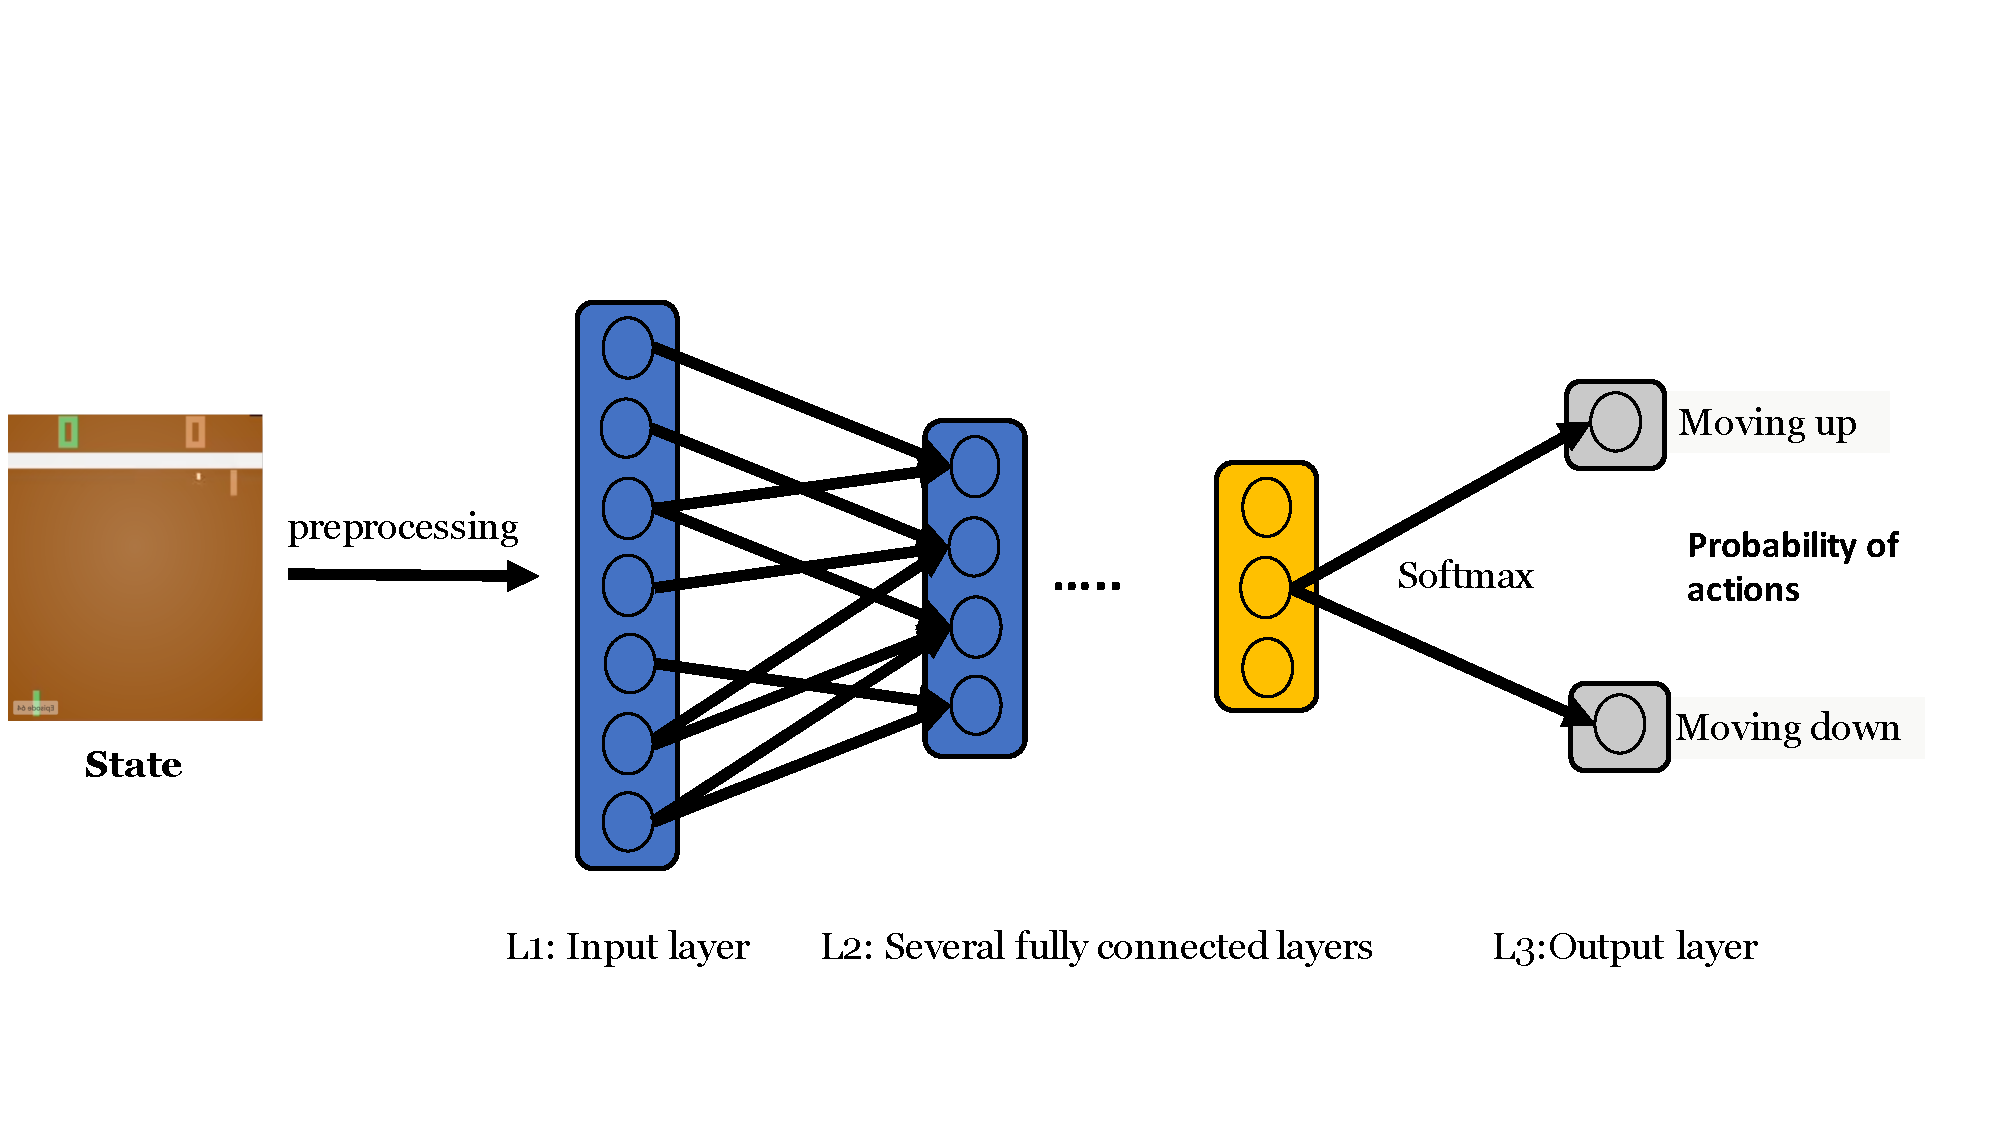
\includegraphics[width=0.49\textwidth]{./fig/policygradient.pdf} \\
\caption{The architecture of policy gradient, using Pong game as an example.}
\label{fig:pg_picture}
\end{figure}


The algorithm of policy gradient is shown in Alg.~\ref{alg:pseudocode Pong}

\begin{algorithm}[H]
\begin{algorithmic}[1]
\STATE Xavier initialization: Initialize the weight parameters
\WHILE{$i=1$ to $N$}
\STATE Preprocessing 
\STATE Policy forward
\STATE Sample action, receive reward
\STATE Policy gradient
\IF{Finish one batch:} 
\STATE Rmsprop/Adam optimizer update
\ENDIF
\ENDWHILE
\end{algorithmic}
\caption{pseudocode for Policy Gradient }
\label{alg:pseudocode Pong}
\end{algorithm}

\subsection{Experiments-Policy Gradient}
%!TEX root = main.tex

The results of policy gradient method on CartPole environment is show
in Figure~\ref{fig:pg_cartpole}. Also, a video illustration can be found
in \href{https://gym.openai.com/evaluations/eval_UaXIaMm1QxPGgW45KHtTA#reproducibility}{this link}.
As we can see in both the video and the figure, the game was solved by 
few hundred episodes. This show the effectiveness of policy gradient methods
and we further train a this model in a more complex environment. 

\begin{figure}[h!]
\centering
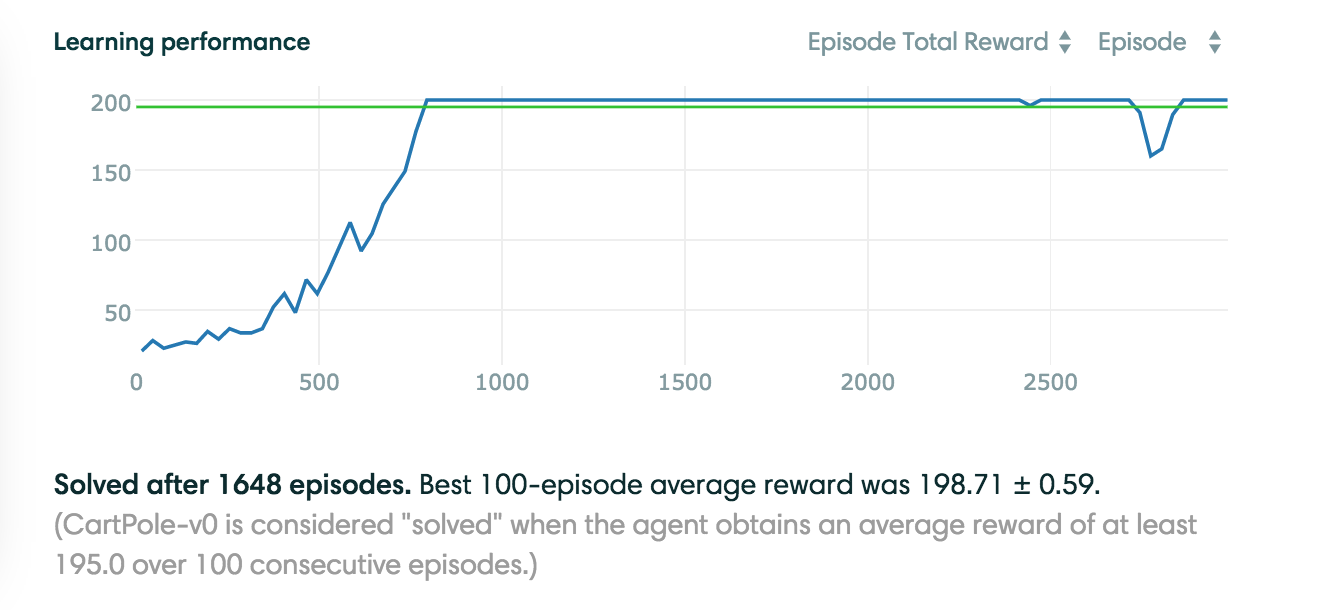
\includegraphics[width=0.49\textwidth]{./fig/pg_cartpole.png} 
\caption{The plot of reward for cartpole game. The x-axis is the number
of episodes it has been trained. The y-axis is the cumulative reward in 
per episode. The higher the better. }
\label{fig:pg_cartpole}
\end{figure}


The performance on Pong game is plot in Figure~\ref{fig:pg_pong} and a video
illustration can be found \href{https://gym.openai.com/evaluations/eval_dODFoXO2S4y5TuUZMX7Nw}{at this link}. As it
shown in the figure, this game requires more than 10000 episodes to get 
a model better than the baseline provided by OpenAI gym. It much more complicated
than the CartPole, since the state and action space is more complex than 
that. The structure of this policy is a single hidden layer with eight
hidden nodes fully connected network and it works. It may perform
better if we use a convolutional network to replace this one, but compared 
the results in dueling DQN, it seems the algorithms of reinforcement learning
itself is more important, other than the specific network architecture. 

\begin{figure}[h!]
\centering
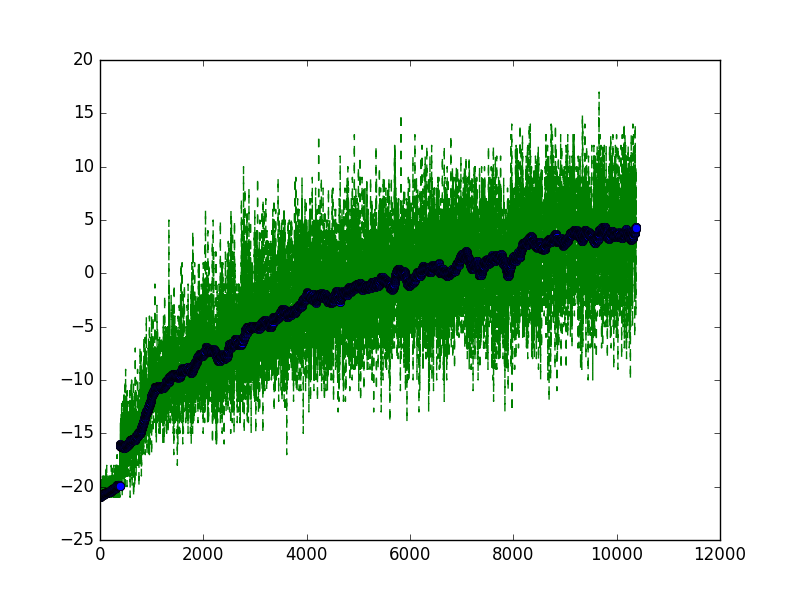
\includegraphics[width=0.49\textwidth]{./fig/pg_pong_rewardsplot.png} 
\caption{The plot of reward for pong game. The x-axis is the number
of episodes it has been trained. The y-axis is the cumulative reward in 
per episode. The higher the better. }
\label{fig:pg_pong}
\end{figure}

% The derive of objective function:

% \begin{equation}
% \begin{split}
% & \max_{\theta} \textbf{E}_a(R(a))  \\
% & \max_{\theta} \sum_a p(a|s; \theta)R(a)
% \end{split}
% \end{equation}
% maximize the expectation of rewards over actions